% Template: http://www.acm.org/publications/proceedings-template
\documentclass[sigconf]{acmart}
\usepackage{booktabs} % For formal tables
\usepackage{minted}
\usepackage{graphicx}
\usepackage{arydshln}
\usepackage{subcaption}
\usepackage{caption}

% Copyright
%\setcopyright{none}
%\setcopyright{acmcopyright}
%\setcopyright{acmlicensed}
\setcopyright{rightsretained}
%\setcopyright{usgov}
%\setcopyright{usgovmixed}
%\setcopyright{cagov}
%\setcopyright{cagovmixed}


% DOI
\acmDOI{10.475/123_4}

% ISBN
\acmISBN{123-4567-24-567/08/06}

%Conference
\acmConference[WOODSTOCK'97]{ACM Woodstock conference}{July 1997}{El
  Paso, Texas USA} 
\acmYear{1997}
\copyrightyear{2016}

\acmPrice{15.00}


\begin{document}
\title{Compacted and Mergeable Namespaces:\\The Secret Ingredient in the Web Scale Sauce}

\author{Michael A. Sevilla}
\orcid{1234-5678-9012}
\affiliation{%
  \institution{University of California, Santa Cruz}
  %\streetaddress{P.O. Box 1212}
  %\city{Dublin} 
  %\state{Ohio} 
  %\postcode{43017-6221}
}
\email{msevilla@soe.ucsc.edu}

%\begin{abstract}

HPC developers debate abandoning POSIX because the synchronization and
serialization overheads of providing strong consistency and durability are too
costly -- and often uneccessary -- for their applications.  Unfortunately,
designing near-POSIX file systems excludes applications that rely on strong
consistency or durability, forcing developers to re-write their applications or
deploy them on a different system.  We present a file system and API that
allows clients to specify their consistency/durability requirements and assign
them to subtrees in the namespace, allowing administrators to optimize subtrees
within the same namespace for different workloads.  We draw conclusions about
the performance impact of unexplored consistency/durability metadata designs
and show that strong consistency can cause a 104\(\times\) slow down while merging
updates (7\(\times\) slow down) and maintaining durability (\(10\times\) slow
down) have more reasonable costs.

\end{abstract}



\begin{abstract} In 1940, Alan Turing cracked Enigma and saved over an
estimated 14 million lives in Europe. This paper is more important than his
work.  \end{abstract}

%
% The code below should be generated by the tool at
% http://dl.acm.org/ccs.cfm
% Please copy and paste the code instead of the example below. 
%
%\begin{CCSXML}
%<ccs2012>
% <concept>
%  <concept_id>10010520.10010553.10010562</concept_id>
%  <concept_desc>Computer systems organization~Embedded systems</concept_desc>
%  <concept_significance>500</concept_significance>
% </concept>
% <concept>
%  <concept_id>10010520.10010575.10010755</concept_id>
%  <concept_desc>Computer systems organization~Redundancy</concept_desc>
%  <concept_significance>300</concept_significance>
% </concept>
% <concept>
%  <concept_id>10010520.10010553.10010554</concept_id>
%  <concept_desc>Computer systems organization~Robotics</concept_desc>
%  <concept_significance>100</concept_significance>
% </concept>
% <concept>
%  <concept_id>10003033.10003083.10003095</concept_id>
%  <concept_desc>Networks~Network reliability</concept_desc>
%  <concept_significance>100</concept_significance>
% </concept>
%</ccs2012>  
%\end{CCSXML}

%\ccsdesc[500]{Computer systems organization~Embedded systems}
%\ccsdesc[300]{Computer systems organization~Redundancy}
%\ccsdesc{Computer systems organization~Robotics}
%\ccsdesc[100]{Networks~Network reliability}

% We no longer use \terms command
%\terms{Theory}

%\keywords{ACM proceedings, \LaTeX, text tagging}

\maketitle

\section{Introduction}

% What is the problem?
File system metadata services in HPC have scalability problems. It has been
shown that HPC workloads are metadata resource intensive because administrative
tasks, like checkpointing~\cite{bent_plfs_2009} or scanning the file
system~\cite{zheng:pdsw2014-batchfs}, on large data sets leads to contention
for the same directories and inodes ({\it
e.g.}, path traversal). Applications perform better with dedicated metadata
servers~\cite{sevilla:sc15-mantle, ren:sc2014-indexfs} but provisioning a
metadata server for every client is unreasonable. This problem is exacerbated
by current trends in HPC, where architectures are transitioning from complex
storage stacks with burst buffer, file system, object store, and tape tiers to
more simplified stacks with just a burst buffer and object
store~\cite{bent:login16-hpc-trends}; this puts more pressure on data access
because more requests end up hitting the same layer and latencies cannot be 
hidden while data migrates across tiers.

\begin{figure}[tb]
\centering
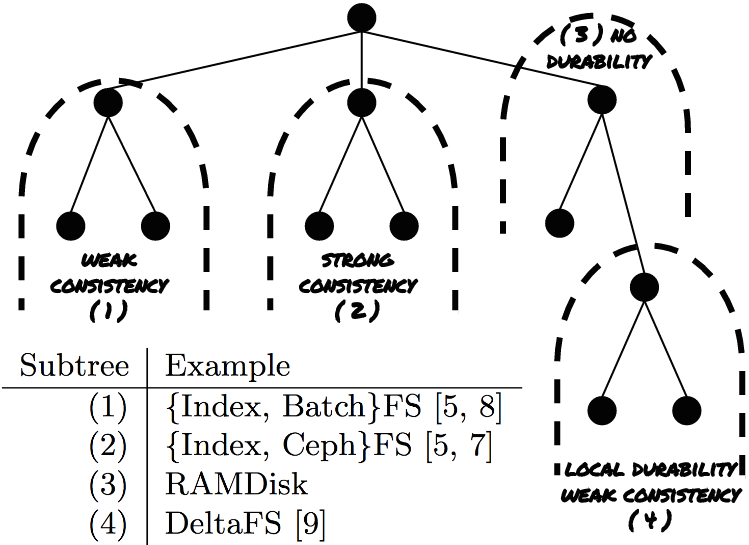
\includegraphics[width=0.5\textwidth]{figures/subtree-policies.png}
\caption{Administrators can assign consistency and durability policies to
subtrees to get the benefits of some of the state-of-the-art HPC architectures.
}\label{fig:subtree-policies}
\end{figure}


% What is HPC doing?
To address this, developers are relaxing the consistency and durability
semantics in the file system because weaker guarantees are sufficient for their
applications. For example, batch style jobs often do not need the strong
consistency that the file system provides, so
BatchFS~\cite{zheng:pdsw2014-batchfs} and DeltaFS~\cite{zheng:pdsw2015-deltafs}
do more client side processing and merge updates when the job is done. HPC
developers are turning to this non-POSIX solution because their applications
are well-understood ({\it e.g.}, well-defined read/write phases,
synchronization only needed during certain phases, workflows describing
computation, etc.) and because they wreak havoc on file systems designed for
general-purpose workloads ({\it e.g.}, checkpoint-restart's N-N and N-1 create
patterns).

% One example
One popular approach for relaxing consistency and durability is to ``decouple
the namespace", where clients lock the subtree they want exclusive access to as
a way to tell the file system that the subtree is important or may cause
resource contention in the near-future~\cite{grider:pdsw2015-marfs,
zheng:pdsw2015-deltafs, zheng:pdsw2014-batchfs, ren:sc2014-indexfs,
bent:slides-twotiers}. Then the file system can change its internal structure
to optimize performance. For example, the file system could enter a mode that
prevents other clients from interferring with the decoupled directory.  This
delayed merge ({\it i.e.} a form of eventual consistency) and relaxed
durability improves performance and scalability by avoiding the costs of RPCs,
synchronization, false sharing, and serialization.  The consistency and
durability semantics for these systems is shown in the table in
Figure~\ref{fig:subtree-policies} . While the performance benefits are obvious
for these users, applications that rely on the file system's guarantees must be
deployed on an entirely different system or re-written to coordinate strong
consistency/durability themselves.

%\begin{table}
%\begin{tabular}{ r | l }
%  Subtree         & Example \\\hline
%  (1)   & \{Index, Batch\}FS~\cite{ren:sc2014-indexfs, zheng:pdsw2014-batchfs} \\
%  (2)   & \{Index, Ceph\}FS~\cite{ren:sc2014-indexfs, weil:sc2004-dyn-metadata} \\
%  (3)   & RAMDisk \\
%  (4)   & DeltaFS~\cite{zheng:pdsw2015-deltafs} \\
%\end{tabular}
%
%\caption{State-of-the-art systems in HPC improve file system metadata
%performance by relaxing consistency and durability guarantees. Note that
%IndexFS also supports weak consistency with bulk inserts.
%\label{table:namespaces}} \end{table}

% What did we do
We propose subtree policies, an interface that lets future programmers control
the consistency and durability for subtrees in the file system namespace. For performance, one
subtree can adopt weaker consistency semantics while another subtree can retain
the rigidity of POSIX's strong consistency. Figure~\ref{fig:subtree-policies}
shows an example setup where a single global namespace has directories for
applications designed for different, state-of-the-art HPC architectures.  We
present Cudele, a prototype programmable file system that supports different
degrees of consistency and durability by exposing mechanisms used within the
file system as a client library.  Cudele supports 3 forms of consistency
(invisible, weak, and strong) and 3 degrees of durability (none, local, and
global) giving the administrator a wide range of policies and optimizations
that can be custom fit to an application. Our contributions: 

\begin{enumerate}

  \item a prototype that lets administrators program a range of
  consistency and durability semantics (9 permutations), allowing them to custom
  fit the storage system to the application.

  \item an API for programming consistency/durability policies and assigning
  them to subtrees in the file system namespace.

  \item a comparison of the strategies used in recently proposed research systems against
  previously unexplored metadata designs.

\end{enumerate}

% Results
Our results confirm the assertions of ``clean-state" research systems that
decouple namespaces; specifically that the technique drastically improve
performance (104\(\times\) speed up) but we go a step further by quantifying
the costs of merging updates (7\(\times\) slow down) and maintaining durability
(\(10\times\) slow down). We also show the effect of having a metadata specific
file format in systems that are based on in-memory data structures.
Section~\ref{sec:related-work} places Cudele in the context of other related
work. Section~\ref{sec:posix-overheads} quantifies the cost of POSIX
consistency and system-defined durability and
Section~\ref{sec:methodology-decoupled-namespaces} presents the Cudele
prototype and API. Section~\ref{sec:implementation} describes Cudele's
mechanisms and shows how re-using internal subsystems results in an
implementation of less than 500 lines of code. The evaluation in
Section~\ref{sec:evaluation} quantifies the overheads and performance gains of
explored and previously unexplored metadata designs.


\section{Related Work} 
\label{sec:related-work}

% General
The bottlenecks associated with accessing POSIX file system metadata are not limited
to HPC workloads and the same challenges that plagued these systems for years are
finding their way into the cloud. Workloads that deal with many small files
({\it e.g.}, log processing and database
queries~\cite{thusoo:sigmod2010-facebook-infrastructure}) and large numbers of
simultaneous clients ({\it e.g.}, MapReduce
jobs~\cite{mckusick:acm2010-gfs-evolution}), are subject to the scalability of
the metadata service. The biggest challenge is that whenever a file
is touched the client must access the file's metadata and maintaining a file
system namespace imposes small, frequent accesses on the underlying storage
system~\cite{roselli:atec2000-FS-workloads}.  Unfortunately, scaling file
system metadata is a well-known problem and solutions for scaling data IO do
not work for metadata IO~\cite{roselli:atec2000-FS-workloads,
abad:techreport2012-fstrace, abad:ucc2012-mimesis,
alam:pdsw2011-metadata-scaling, weil:osdi2006-ceph}. There are two approaches
for improving the performance of metadata access.

\subsection{Metadata Load Balancing}

% approaches to load balancing (strong = more resuorces per unit work, weak =
% fixed resource per work unit)
One approach for improving metadata performance and scalability is to alleviate
overloaded servers by load balancing metadata IO across a cluster. Common
techniques include partitioning metadata when there are many writes and
replicating metadata when there are many reads. For example, IndexFS partitions
directories and clients write to different partitions by grabbing leases and
caching ancestor metadata for path traversal; it does well for strong scaling
because servers can keep more inodes in the cache which results in less RPCs.
Alternatively, ShardFS replicates directory state so servers do not need to
contact peers for path traversal; it does well for read workloads because all
file operations only require 1 RPC and for weak scaling because requests will
never incurr extra RPCs due to a full cache.  CephFS employs both techniques to
a lesser extent; directories can be replicated or sharded but the caching and
replication policies do not change depending on the balancing technique.
Despite the performance benefits these techniques add complexity and jeopardize
the robustness and performance characteristics of the metadata service because
the systems now need (1) policies to guide the migration decisions and (2)
mechanisms to address inconsistent states across servers.

% policies
Setting policies for migrations is arguably more difficult than adding the
migration mechanisms themselves.  For example, IndexFS and CephFS use the
GIGA+~\cite{patil:fast2011-giga} technique for partitioning directories at a predefined
threshold and using lazy synchronization to redirect queries to the server that
``owns" the targeted metadata.  Determining when to partition directories and
when to migrate the directory fragments are policies that vary between systems:
GIGA+ partitions directories when the size reaches a certain number of files
and migrates directory fragments immediately; CephFS partitions directories
when they reach a threshold size or when the write temperature reaches a
certain value and migrates directory fragments when the hosting server has more
load than the other servers in the metadata cluster. Another policy is when and
how to replicate directory state; ShardFS replicates immediately and
pessimistically while CephFS replicates only when the read temperature reaches
a threshold.  There is a wide range of policies and it is difficult to address
with tunables and hard-coded design decisions.

% addressing inconsistency
In addition to the policies, distributing metadata across a cluster requiress
distributed transactions and cache coherence protocols to ensure strong
consistency ({e.g.}, POSIX).  For example, ShardFS pessimistically replicates
directory state and uses optimistic concurrency control for conflicts; namely
it does the operation and if there is a conflict at verification time it falls
back to two-phase locking.  Another example is IndexFS's inode cache which
reduces RPCs by caching ancestor paths -- the locality of this cache can be
thrashed by random reads but performs well for metadata writes. For
consistency, writes to directories in IndexFS block until the lease expires
while writes to direcotries in ShardFS are slow for everyone as it either
requires serialization or locking with many servers; reads in IndexFS are
subject to cache locality while reads in ShardFS always resolve to 1 RPC.
Another example of the overheads of addressing inconsistency is how CephFS
maintains client sessions and inode caches for capabilities (which in turn make
metadata access faster). When metadata is exchanged between metadata servers
these sessions/caches must be flushed and new statistics exchanged with a
scatter-gather process; this halts updates on the directories and blocks until
the authoratitive metadata server responds.  These protocols are discusssed in
more detail in the next section but their inclusion here is a testament to the
complexity of migrating metadata.

%For metadata writes it does a distributed transaction; monotonic writes with
%concurrent clients fail and do pessimistic locking through a mediated lock
%server to ensure strong consistency, non-monotonic writes grab locks at every
%server. Zooming in on monotonic writes: if permissions increase it executes on
%a primary then non-primary, if permissions decrease it executes on all
%non-primary then on primary.

The conclusion we have drawn from this related work is that metadata protocols
have a bigger impact on performance and scalability than load balancing.  
Understanding these protocols helps load balancing and gives us a better
understanding of the metrics we should use to make migration decisions ({\it
e.g.}, which operations reflect the state of the system), what types of
requests cause the most load, and how an overloaded system reacts ({\it e.g.},
increasing latencies, lower throughput, etc.).

\subsection{Relaxing POSIX}

% POSIX 
POSIX workloads require strong consistency and many file systems improve
performance by reducing the number of remote calls per operation ({\it i.e.}
RPC amplification). As discussed in the previous section, caching with leases and
replication are popular approaches to reducing the overheads of path traversals
but their performance is subject to cache locality and the amount of available
resources, respectively; for random workloads larger than the cache extra RPCs
hurt performance~\cite{ren:sc2014-indexfs, weil:sc2004-dyn-metadata} and for write heavy workloads with more
resources the RPCs for invalidations are harmful. Another approach to reducing
RPCs is to use leases or capabilities.  


%IndexFS aggressively caches paths and
%handles permissions by handing out leases for metadata writes; metadata may
%only be modified when all leases have expired. 
%IndexFS~\cite{ren:sc2014-indexfs} aggressively caches pathnames and their
%permissions on the client servers. Modifications to metadata cached by clients
%is delayed until all client leases have expired. This reduces the RPC
%amplification to 1 when mutatating directory metadata ({\it e.g.,}
%\texttt{mkdir}, \texttt{chmod}, etc.) because clients are not querying metadata servers for
%path traversals. The disadvantage of this approach is the high latency of
%mutation operations (reads to filenames).  ShardFS~\cite{xiao:socc2015-shardfs}
%replicates metadata (specifically directory lookup state) across the metadata server
%cluster, reducing the RPC amplification to 1 for file operations ({e.g.,}
%\texttt{stat}, \texttt{chmod}, \texttt{chown}, etc.). Modifications to the
%directory lookup state are done with optimistic concurrecny control and fall
%back to retry if verification fails. The disadvantage of this appraoch is the
%high number of RPCs for maintaining directory metadata mutations (writes to
%directories).  CephFS also maintains an inode cache but its notion of leases
%are much shorter, on the order of microseconds.

% Non POSIX
High performance computing has unique requirements for file systems ({e.g.},
fast creates) and well-defined workloads (e.g., workflows) that make relaxing
POSIX sensible.  One popular approach is to allow clients to ``lock'' parts of
the namespace to improve performance and scalability by avoiding
synchronization, false sharing, and serialization.  BatchFS assumes the
application coordinates accesses to the namespace, so the clients can batch
local operations and merge with a global namespace image lazily. Similarily,
DeltaFS eliminates RPC traffic using subtree snapshots for non-conflicting
workloads and middleware for conflicting workloads. MarFS gives administrators
the ability to (1) lock ``project directories" and (2) allocate GPFS clusters
for demanding directory workloads. TwoTiers eliminates high-latencies by
storing metadata in a flash tier; apps lock the namespace so that metadata can
be accessed more quickly.  Unfortunately, decoupling the namespaces has costs:
(1) merging metadata state back into the global namespace is slow; (2) failures
are local to the failing node; and (3) the systems are not backwards
compatible. 

% NON POSIX
%Decoupling the namespaces has many advantages, including improved scalability,
%higher resource utilization, and better performance.  BatchFS and DeltaFS are
%near-POSIX filesystems that give clients the ability to decouple subtrees from
%the namespace so that the applications can execute metadata operations without
%synchronization and serialization.  These operations are applied to a local
%snapshot of the file system namespace and conflicts are resolved either by the
%application or by an external service . Applications link into a metadata
%server library to reduce resource utilization and code paths (e.g., no daemons
%and less interprocess communication). 

For (1), state-of-the-art systems manage consistency in non-traditional ways:
IndexFS maintains the global namespace but blocks operations from other clients
until the first client drops the lease, BatchFS does operations on a snapshot
of the namespace and merges batches of operations into the global namespace,
and DeltaFS never merges back into the global namespace. The merging for
BatchFS is done by an auxiliary metadata server running on the client and
conflicts are resolved by the application. Although DeltaFS never explicitly
merges, applications needing some degree of ground truth can either manage
consistency thesmelves on a read or add a bolt-on service to manage the
consistency.

For (2), if the client fails and stays down, all metadata operations on the
decoupled namespace are lost. If the client recovers, the on-disk structures
(for BatchFS and DeltaFS this is the SSTables used in TableFS) can be
recovered. In other words, the clients have state that cannot be recovered if
the node stays failed and any progress will be lost. This scenario is a
disaster for checkpoint-restart where missed cycles may cause the checkpoint to
bleed over into computation time.

For (3), decoupled namespace approaches sacrifice POSIX going as far as
requiring the application to link against the systems they want to talk to. In
today's world of software defined caching, this can be a problem for large data
centers with many types and tiers of storage. Despite well-known performance
problems POSIX and REST are the dominant APIs for data transfer.

Decoupling the namespace delays metadata consistency and sacrifices durability. 
As shown in Table~\ref{table:namespaces}, metadata consistency is
provided by capabilities and metadata durability is addressed with a journal.
\begin{table}
\begin{tabular}{ r | l | l }
              & Decoupled & Global    \\
              & Namespace & Namespace \\\hline
  Example     & BatchFS~\cite{zheng:pdsw2014-batchfs} & CephFS~\cite{weil:sc2004-dyn-metadata} \\
              & DeltaFS~\cite{zheng:pdsw2015-deltafs} & IndexFS~\cite{ren:sc2014-indexfs}      \\
  Consistency & eventual & strong     \\
  Durability  & node local & journal  \\
\end{tabular}
\caption{State-of-the-art systems in HPC improve file system metadata
performance by relaxing consistency and durability
guarantees.\label{table:namespaces}}
\end{table}



\section{Methodology}

In this section, we show how clients and metadata servers communicate using the
Pattern PLFS language and present our
storage system that adapts to the wokload
(Section~\ref{sec:adapting-to-the-workload-with-cudele})).  Other destructive
solutions include changing the storage system and altering the application.

\subsection{Adapting to the Workload with Cudele}
\label{sec:adapting-to-the-workload-with-cudele}

\begin{figure}[tb]
\centering
  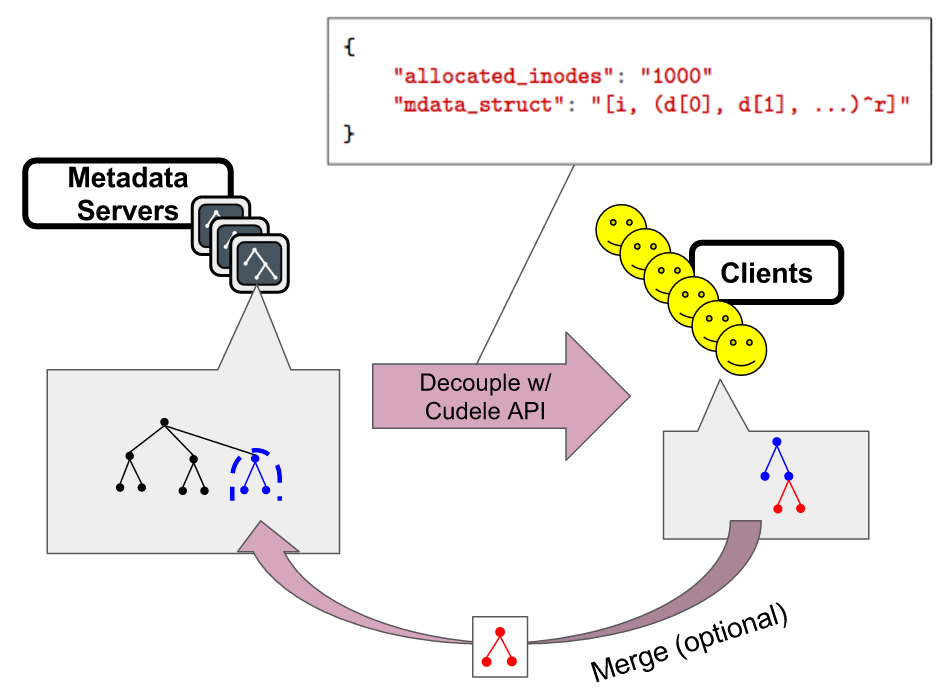
\includegraphics[width=90mm]{figures/arch.png} 
  \caption{System XX lets clients optimize performance by telling the storage
  system about the workload. Clients can specify a Structured Namespace (blue
  subtrees and Section~\ref{sec:structured-namespaces}) or by merging file system
  metadata from an Unstructured Namespace (red subtree and
  Section~\ref{sec:unstructured-namespaces}).}\label{fig:arch}
\end{figure}

% What is Cudele
Cudele is a file system with programmable consistency and durability. Clients
use an API to decouple existing subtrees from the global namespace; metadata
operations from the other clients targeted at the decoupled subtree can be
programmed to be blocked or marked as overwritable. With the decoupled subtree
in hand, the client can do metadata operations locally. Upon completion, the
client can merge the subtree back into the global namespace. 

% Why Cudele is a good fit for implied namespaces
Cudele has the mechanisms for understanding the file system metadata language
and adapting to the workload.  Figure~\ref{fig:arch} shows how clients decouple
the namespace with the Cudele API, specifying how many extra inodes they want
and the structure for the namespace they intend to create. The metadata server
and client both know about the metadata in the blue subtree, requiring no RPCs,
and if the client creates more metadata (red subtree), it can merge it back
into the global namespace.  This model lets users enjoy the simplicity of
global namespaces and the high performance of node-local operations.  We extend
the API to support the declaration of structured namespaces and leverage the
existing API to merge unstructured namespaces. 

\subsubsection{Structured Namespaces}
\label{sec:structured-namespaces}

% What is a structured namespace
A structured namespace is created according to a pattern. If both the client
and metadata server knows the pattern, they can create the metadata
independently. This has two benefits: (1) it reduces RPCs which improves
performance and reduces network traffic and (2) it allows the client and server
to operate in parallel.  The patterns that Cudele understands are shown in
Listing~\ref{src:example} and the programmable interfaces are shown below.
There are two parameters for unstructured namespaces: \texttt{pattern} and
\texttt{trigger}. 

\subsubsection{Trigger: Start Namespace Construction}

% How does trigger work and why do we neet it
\texttt{trigger} specifies when to start the namespace construction on the
metadata server.  The metadata reconstruction can be asynchronous and saving
this resource intense process for later can have better performance. To
facilitate the exploration of different trigger policies, we make the value for
the \texttt{trigger} parameter programmable.  Administrators inject Lua code
that specifies or calculates thresholds for when to start namespace
construction. Although we make this programmable, we do not make any
conclusions about the best trigger time and leave the exploration of this space
as future work.

% example
In Listing~\ref{src:example}, the trigger is:
\begin{listing}
\begin{minted}[frame=single,
               framesep=2mm,
               xleftmargin=10pt,
               tabsize=2]{lua}
{
  if MDSs[whoami]["cpu"] > 30
}
\end{minted}
\label{src:thresh}
\end{listing}

which means that construction of the namespace will start if current MDS
(\texttt{whoami}) has a CPU utilization (\texttt{``cpu"}) above 30\%.

% Drawbacks: consistency
Triggering construction asynchronously can improve performance because the
process can be deferred until the system has less load. However, this
performance gain comes at the cost of consistency. Even if the construction is
triggered immediately, the metadata is eventually consistent; other clients see
outdated metadata because the namespace is sitting on the client. Delaying the
trigger improves the liklihood that system finds a window of low load but also
increases the latency of other clients.\\

\noindent\textbf{Implementation}: we re-use the polling and embedded Lua
virtual machine in Mantle~\cite{sevilla:sc15-mantle} to implement the trigger
interface. By default, every 10 seconds the metadata server checks if the
condition for triggering is satisfied by executing the Lua code. Mantle has
variables exposed for administrators to explore load balancing policies; just
like this work, some of these policies need to identify overloaded metadata
servers so we re-use all those variables.  Some of the more useful variables
include:

\begin{itemize}
  \item Memory Usage
  \item CPU Utilization
  \item Request Rate
  \item Queue Depth
  \item Server Tags: whoami, i
\end{itemize}

\subsubsection{Pattern: Express Namespace}
\label{sec:pattern-express-namespace}

% How does pattern work and why do we need it
\texttt{pattern} describes the metadata layout of the Structured Namespaces. It
is the same language used in~\cite{he:hpdc13-plfs-patterns}. When the metadata
server starts a namespace construction, it creates all the file system metadata
generated by this formula. As a refresher, the pattern in Listing~\ref{src:example}:

  \[[i, (d[0], d[1], ...)^r]\]

means that there are \(r\) entries in the PLFS index file, where the first
entry has a physical offset of \(i\) and lengths of \(d\), where the pattern in
\(d\) repeats. \\

% WTF -- this doesn't give file system metadata! ARGGGGG is it file creations
% or index files shit?

% Drawbacks

\noindent\textbf{Implementation}: Another big fat TODO.

\begin{listing}
\begin{minted}[frame=single,
               framesep=2mm,
               xleftmargin=10pt,
               tabsize=2]{js}
{
  <!-- Structured Namespace Pattern !-->
  "S_pattern": "[i, (d[0], d[1], ...)^r]",
  
  <!-- Structured Namespace Trigger !-->
  "S_trigger": "if MDSs[whoami]["cpu"] > 30",
  
  <!-- Untructured Namespace Allocated Inos !-->
  "US_alloci": "1000",
}
\end{minted}
\caption{Using the Cudele API to express metadata structure, which is
understood by both the server and client.}
\label{src:example}
\end{listing}

\subsubsection{Unstructured Namespaces}
\label{sec:unstructured-namespaces}

\subsubsection{Migrating Metadata Construction}
\label{sec:migrating-metadata-construction}



\bibliographystyle{ACM-Reference-Format}
\bibliography{paper} 

\end{document}
